\section{Comparison of a PMU-based approach and the draft requirements approach using tests from two of Statkraft's power plants Paper IV}
\begin{frame}
	\frametitle{Motivation}
	\begin{itemize}[<+->]
		\item Relate the results from Paper III and the new requirements.
		\item Test the methods on more real datasets.
		\item Demonstrate that industry proposed tests can be done easier.
		\item Less theoretical presentation in a more industry focused conference.
	\end{itemize}
\end{frame}
\begin{frame}
	\frametitle{The new requirements}
	\begin{columns}
		\begin{column}{0.5\textwidth}
			\begin{itemize}[<+->]
				\item Puts requirements on an aggregated system model.
					\includegraphics<1>{./pictures/req_sys.tikz}
				\item Stability requirement
				\begin{align}
						M_s &= \max |\frac{1}{1+G_{p}(j\Omega)G_{J}(j\Omega)}|\nonumber \\
							&= \max |S(j\Omega)|
				\end{align}
				\item Performance requirement
				\begin{equation}
					|G_1(j\Omega)| <\frac{\sigma_{\omega_{req}}}{\sqrt{\phi_{P_{e}}(j\Omega)}}
				\end{equation}
				\item Requirement per plant stated using a per unit conversion
			\end{itemize}
		\end{column}
		\begin{column}{0.5\textwidth}
			\begin{figure}
				\includegraphics<2>[width=\textwidth]{./pictures/nyquist_L.tikz}
			\end{figure}
		\end{column}
	\end{columns}
\end{frame}
\begin{frame}
	\frametitle{Alternative requirements}
	\begin{columns}
		\begin{column}{0.5\textwidth}
				\begin{itemize}[<+->]
				\item Place requirements directly on one power plant.
				\includegraphics<1>{./pictures/sys.tikz}
				\includegraphics<1>{./pictures/req_sys.tikz}
				\item We already have an estimate of $G_1(s)$.
				\item We need to find $S(s)$
			\end{itemize}
		\end{column}
		\begin{column}{0.5\textwidth}
			\begin{figure}
				\includegraphics<2>[width=\textwidth]{./pictures/PMU_bode.tikz}
			\end{figure}
		\end{column}
	\end{columns}
\end{frame}
\begin{frame}
	\frametitle{Estimating $S(s)$}
	\begin{itemize}[<+->]
		\item
		\begin{equation} 
			G_1(s) = G_J(s)S(s)
		\end{equation}
		\item
		\begin{equation}
			G_J(s) = \frac{1}{2Hs+K_d}
		\end{equation}
		\item
		\begin{equation}
			2H>>K_d
		\end{equation}
		\item
		\begin{equation}
			S(s) \approx 2HsG_1(s)
		\end{equation}
		\item Need to estimate $H$
	\end{itemize}
\end{frame}
\begin{frame}
	\frametitle{Estimating $H$}
	\begin{figure}
			\includegraphics[width=0.9\textwidth]{./pictures/transf_comp.tikz}
	\end{figure}
\end{frame}
\begin{frame}
	\frametitle{Dataset from Statkraft}
	\begin{itemize}[<+->]
		\item One of Norway's biggest power producers.
		\item They performed the tests from the draft requirements
		\item By chance I had PMU measurements from the same plant.
		\end{itemize}
		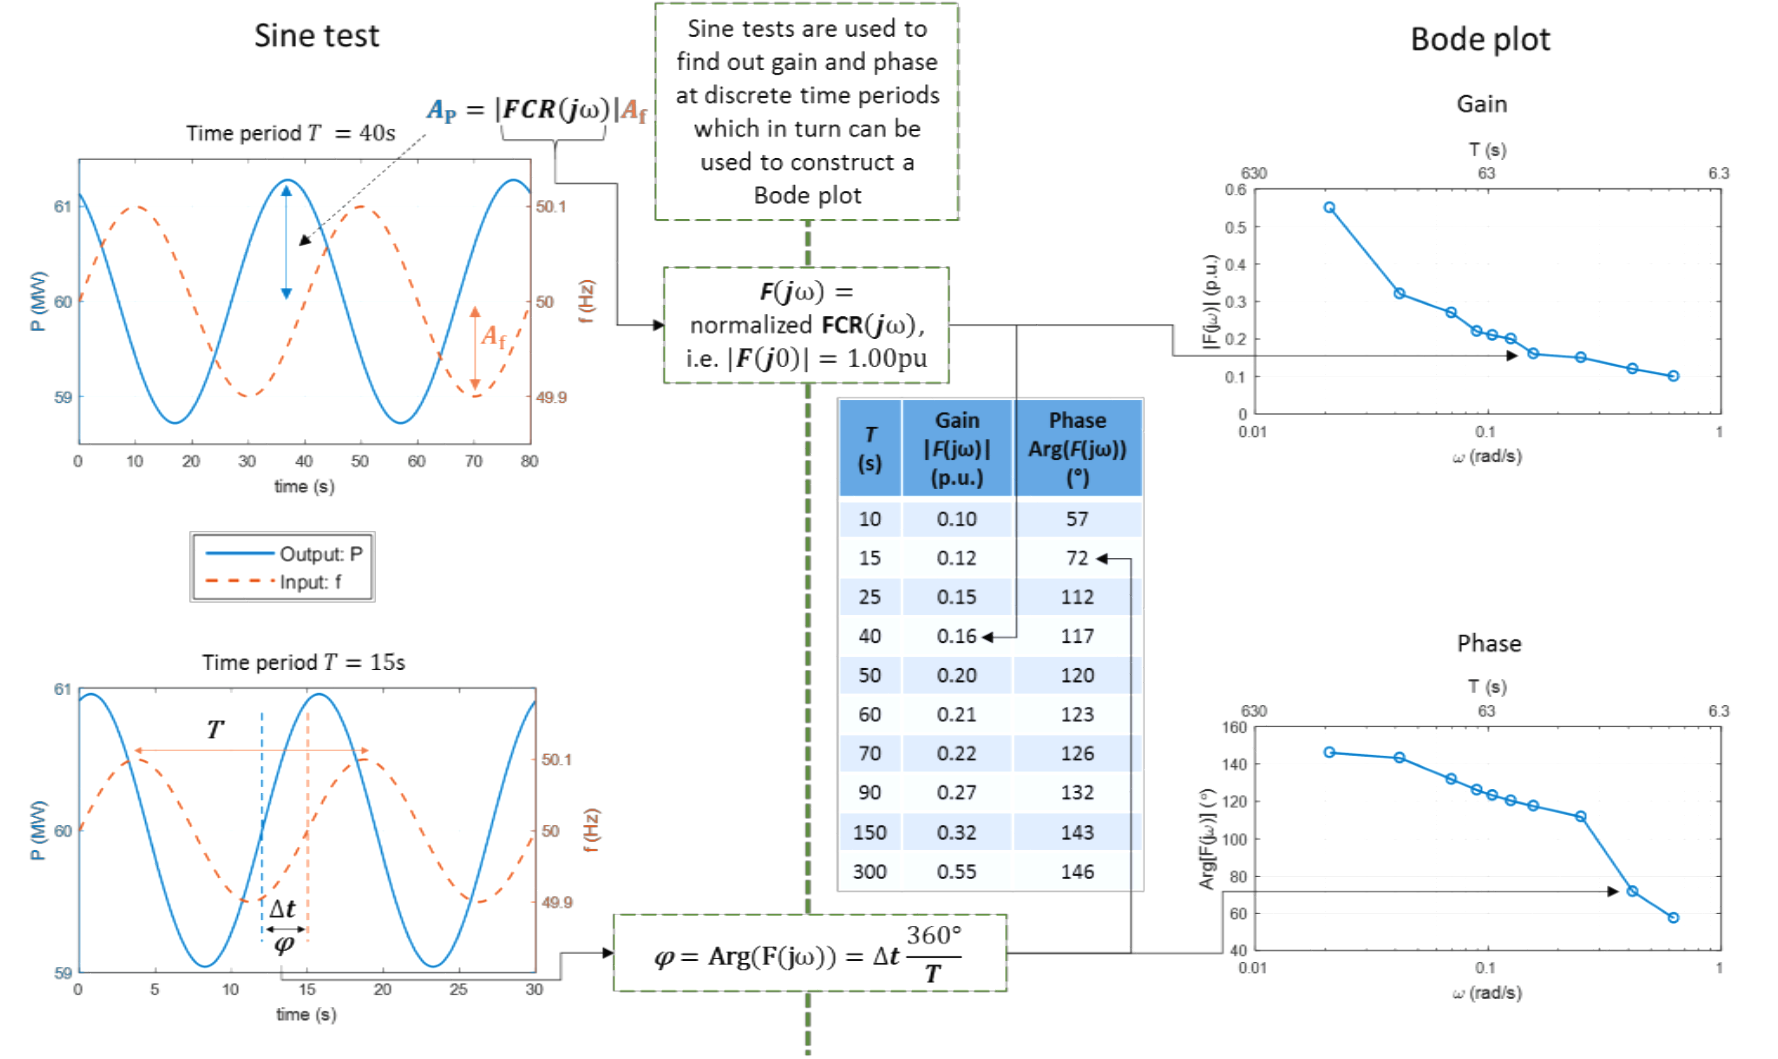
\includegraphics[width=0.8\textwidth]{./pictures/tests.png}
\end{frame}
\begin{frame}
	\frametitle{Single line diagram of the plant}
	\begin{figure}
		\includegraphics{./pictures/plant_sld.tikz}
	\end{figure}
\end{frame}
\begin{frame}
	\frametitle{Datasets used}
	\begin{figure}
			\includegraphics[width=0.8\textwidth]{./pictures/signals_step.tikz}
	\end{figure}
\end{frame}
\begin{frame}
	\frametitle{Estimated sensitivity functions}
		\begin{figure}[tb]
			\includegraphics[width=0.8\textwidth]{./pictures/S_aura.tikz}
		\end{figure}
\end{frame}
\begin{frame}
	\frametitle{Estimated $G_1(s)$}
		\begin{figure}[tb]
			\includegraphics[width=0.8\textwidth]{./pictures/G1_aura.tikz}
		\end{figure}
\end{frame}
\begin{frame}
	\frametitle{Can the industry proposed tests be done easier?}
	\begin{figure}
		\includegraphics<1->[width=0.6\textwidth]{./pictures/aura_signals.tikz}
	\end{figure}
	\begin{figure}
		\includegraphics<1>[width=0.6\textwidth]{./pictures/frd.tikz}
		\includegraphics<2>[width=0.6\textwidth]{./pictures/frd_vs_bj.tikz}
	\end{figure}
\end{frame}
\begin{frame}
	\frametitle{Control system data in closed loop}
	\begin{figure}
		\includegraphics<1->[width=0.4\textwidth]{./pictures/Grytten_signals.tikz}
	\end{figure}
	\begin{figure}
		\includegraphics<1>[width=0.6\textwidth]{./pictures/Grytten_new_PID.tikz}
		\includegraphics<2>[width=0.6\textwidth]{./pictures/Grytten_R_5.tikz}
		\includegraphics<3>[width=0.6\textwidth]{./pictures/Grytten_windows.tikz}
	\end{figure}
	\begin{itemize}
			\item<4>[]
			\begin{tabular}{c c c c c}
			\toprule
			Droop & $60\mathrm{min}$ & $45\mathrm{min}$ & $30\mathrm{min}$ & $15\mathrm{min}$ \\
			\midrule
			$10\%$ & $9.5\%$ & $9.5\%$ & $9.5\%$ & $9.5\%$ \\
			$6\%$ & $6.2\%$ & $6.0\%$ & $5.9\%$ & $6.1\%$ \\
			$5\%$ & $4.9\%$ & $4.9\%$ & $5.0\%$ & $5.1\%$ \\
			$3\%$ & $3.1\%$ & $3.1\%$ & $3.1\%$ & $2.9\%$ \\
			$2\%$ & $2.0\%$ & $1.8\%$ & $1.8\%$ & $1.7\%$\\
			\bottomrule
		\end{tabular}
	\end{itemize}
\end{frame}
\begin{frame}
	\frametitle{Main Contributions}
	\begin{itemize}
		\item Proposal for alternative tests.
		\item Demonstrating that the proposed methods can detect parameter changes.
		\item Demonstrated that the industry proposed tests can be done easier.
	\end{itemize}
\end{frame}
